%package list
\documentclass{article}
\usepackage[top=3cm, bottom=3cm, outer=3cm, inner=3cm]{geometry}
\usepackage{multicol}
\usepackage{graphicx}
\usepackage{url}
%\usepackage{cite}
\usepackage{hyperref}
\usepackage{array}
%\usepackage{multicol}
\newcolumntype{x}[1]{>{\centering\arraybackslash\hspace{0pt}}p{#1}}
\usepackage{natbib}
\usepackage{pdfpages}
\usepackage{multirow}
\usepackage[normalem]{ulem}
\useunder{\uline}{\ul}{}
\usepackage{svg}
\usepackage{xcolor}
\usepackage{listings}
\lstdefinestyle{ascii-tree}{
    literate={├}{|}1 {─}{--}1 {└}{+}1 
  }
\lstset{basicstyle=\ttfamily,
  showstringspaces=false,
  commentstyle=\color{red},
  keywordstyle=\color{blue}
}
%\usepackage{booktabs}
\usepackage{caption}
\usepackage{subcaption}
\usepackage{float}
\usepackage{array}

\newcolumntype{M}[1]{>{\centering\arraybackslash}m{#1}}
\newcolumntype{N}{@{}m{0pt}@{}}


%%%%%%%%%%%%%%%%%%%%%%%%%%%%%%%%%%%%%%%%%%%%%%%%%%%%%%%%%%%%%%%%%%%%%%%%%%%%
%%%%%%%%%%%%%%%%%%%%%%%%%%%%%%%%%%%%%%%%%%%%%%%%%%%%%%%%%%%%%%%%%%%%%%%%%%%%
\newcommand{\itemEmail}{lluquecon@unsa.edu.pe fgarambel@unsa.edu.pe jajra@unsa.edu.pe wchoquehuancab@unsa.edu.pe}
\newcommand{\itemStudent}{Luis Guillermo Luque Condori, Fernando Miguel Garambel Marín, William Herderson Choquehuanca Berna, Jeans Anthony Ajra Huacso}
\newcommand{\itemCourse}{Laboratorio de P.Web}
\newcommand{\itemCourseCode}{}
\newcommand{\itemSemester}{III}
\newcommand{\itemUniversity}{Universidad Nacional de San Agustín de Arequipa}
\newcommand{\itemFaculty}{Facultad de Ingeniería de Producción y Servicios}
\newcommand{\itemDepartment}{Departamento Académico de Ingeniería de Sistemas e Informática}
\newcommand{\itemSchool}{Escuela Profesional de Ingeniería de Sistemas}
\newcommand{\itemAcademic}{2024 - A}
\newcommand{\itemInput}{Del 18 de junio de 2024}
\newcommand{\itemOutput}{Al 22 de junio de 2024}
\newcommand{\itemPracticeNumber}{09}
\newcommand{\itemTheme}{Angular}
%%%%%%%%%%%%%%%%%%%%%%%%%%%%%%%%%%%%%%%%%%%%%%%%%%%%%%%%%%%%%%%%%%%%%%%%%%%%
%%%%%%%%%%%%%%%%%%%%%%%%%%%%%%%%%%%%%%%%%%%%%%%%%%%%%%%%%%%%%%%%%%%%%%%%%%%%

\usepackage[english,spanish]{babel}
\usepackage[utf8]{inputenc}
\AtBeginDocument{\selectlanguage{spanish}}
\renewcommand{\figurename}{Figura}
\renewcommand{\refname}{Referencias}
\renewcommand{\tablename}{Tabla} %esto no funciona cuando se usa babel
\AtBeginDocument{%
	\renewcommand\tablename{Tabla}
}

\usepackage{fancyhdr}
\pagestyle{fancy}
\fancyhf{}
\setlength{\headheight}{30pt}
\renewcommand{\headrulewidth}{1pt}
\renewcommand{\footrulewidth}{1pt}
\fancyhead[L]{\raisebox{-0.2\height}{
\includegraphics[width=3cm]{img/logo_episunsa.png}}}
\fancyhead[C]{\fontsize{7}{7}\selectfont	\itemUniversity \\ \itemFaculty \\ \itemDepartment \\ \itemSchool \\ \textbf{\itemCourse}}
\fancyhead[R]{\raisebox{-0.2\height}{
\includegraphics[width=1.2cm]{img/logo_abet}}}
\fancyfoot[L]{Luis, Fernando, Anthony, William}
\fancyfoot[C]{\itemCourse}
\fancyfoot[R]{Página \thepage}

% para el codigo fuente
\usepackage{listings}
\usepackage{color, colortbl}
\definecolor{dkgreen}{rgb}{0,0.6,0}
\definecolor{gray}{rgb}{0.5,0.5,0.5}
\definecolor{mauve}{rgb}{0.58,0,0.82}
\definecolor{codebackground}{rgb}{0.95, 0.95, 0.92}
\definecolor{tablebackground}{rgb}{0.8, 0, 0}

\lstset{frame=tb,
	language=bash,
	aboveskip=3mm,
	belowskip=3mm,
	showstringspaces=false,
	columns=flexible,
	basicstyle={\small\ttfamily},
	numbers=none,
	numberstyle=\tiny\color{gray},
	keywordstyle=\color{blue},
	commentstyle=\color{dkgreen},
	stringstyle=\color{mauve},
	breaklines=true,
	breakatwhitespace=true,
	tabsize=3,
	backgroundcolor= \color{codebackground},
}

\begin{document}
	
	\vspace*{10px}
	
	\begin{center}	
		\fontsize{17}{17} \textbf{ Informe de Laboratorio \itemPracticeNumber}
	\end{center}
	\centerline{\textbf{\Large Tema: \itemTheme}}
	%\vspace*{0.5cm}	

	\begin{flushright}
		\begin{tabular}{|M{2.5cm}|N|}
			\hline 
			\rowcolor{tablebackground}
			\color{white} \textbf{Nota}  \\
			\hline 
			     \\[30pt]
			\hline 			
		\end{tabular}
	\end{flushright}	

	\begin{table}[H]
		\begin{tabular}{|x{4.7cm}|x{4.8cm}|x{4.8cm}|}
			\hline 
			\rowcolor{tablebackground}
			\color{white} \textbf{Estudiante} & \color{white}\textbf{Escuela}  & \color{white}\textbf{Asignatura}   \\
			\hline 
			{\itemStudent \par \itemEmail} & \itemSchool & {\itemCourse \par Semestre: \itemSemester \par  \itemCourseCode}     \\
			\hline 			
		\end{tabular}
	\end{table}		
	
	\begin{table}[H]
		\begin{tabular}{|x{4.7cm}|x{4.8cm}|x{4.8cm}|}
			\hline 
			\rowcolor{tablebackground}
			\color{white}\textbf{Laboratorio} & \color{white}\textbf{Tema}  & \color{white}\textbf{Duración}   \\
			\hline 
			\itemPracticeNumber & \itemTheme & 04 horas   \\
			\hline 
		\end{tabular}
	\end{table}
	
	\begin{table}[H]
		\begin{tabular}{|x{4.7cm}|x{4.8cm}|x{4.8cm}|}
			\hline 
			\rowcolor{tablebackground}
			\color{white}\textbf{Semestre académico} & \color{white}\textbf{Fecha de inicio}  & \color{white}\textbf{Fecha de entrega}   \\
			\hline 
			\itemAcademic & \itemInput &  \itemOutput  \\
			\hline 
		\end{tabular}
	\end{table}

	\clearpage




	\section{REPOSITORIO GitHub}

	\begin{itemize}
		\item \url{https://github.com/nuevo637/Lab-09-Angular}
	\end{itemize}
	
	\section{Videos}
	\begin{itemize}
		\item \url{https://flip.com/s/cK4x1VbL49nw}
		\item \url{https://flip.com/s/cH62CS-ZBK3q}
		\item \url{L}
		\item \url{W}
	\end{itemize}

	\section{Introducción Angular}
	\begin{itemize}
		\item Primero tenemos que tener una version de TypeSript de la 17 en adelante para poder instalar Angular.
		\item Luego usamos los siguientes comandos para instalarlo y verificar la instalción.
		\begin{lstlisting}[language=bash,caption={Comandos para instalar Angular}][H]
			$ npm install -g @angular/cli
			$ ng varsion
		\end{lstlisting}
		\item si nos sale la siguiente imangen angular estará instalado
		\begin{figure}[H]
			\centering
			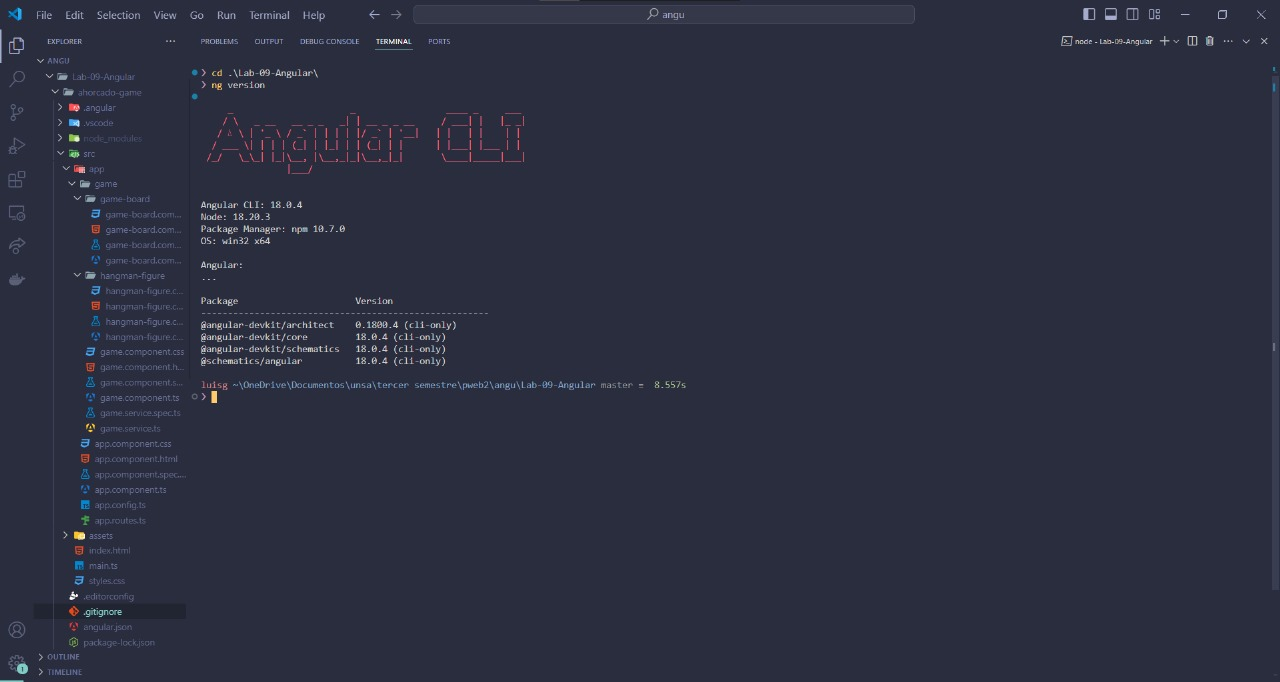
\includegraphics[width=0.8\textwidth,keepaspectratio]{img/instalamosANgular.jpg}
			%\includesvg{img/automata.svg}
	
		\end{figure}
		\item para crear un proyecto en angular usamos la siguiente linea de comandos.
		\begin{lstlisting}[language=bash,caption={Crear Proyecto en Angular}][H]
			$ ng new ahorcado-game
		\end{lstlisting}
		\item Luego observaremos un archivo padre que seria nuestra app donde tendremos estilos que son genericos, html y un archivo de componentes que nos ayudaran a juntar mas componentes después.
		\item Los componentes nos ayudan a dar valores y lógica a nuestra página web.
		\item Ahora para crear un componente usaremos la siguiente línea de comandos.
		\begin{lstlisting}[language=bash,caption={Crear Componentes}][H]
			$ ng generate component game-board
			$ ng generate component hangman-figure 
		\end{lstlisting}
		\item Esto nos ayuda para poder trabajar por partes y no tenerlo todo en un solo código ademas al momento de cambiar estilos es mas fácil.
		\item En nuestro caso usamos 2 componentes uno para la lógica y otro para crear el muñeco de ahorcado.
		\begin{figure}[H]
			\centering
			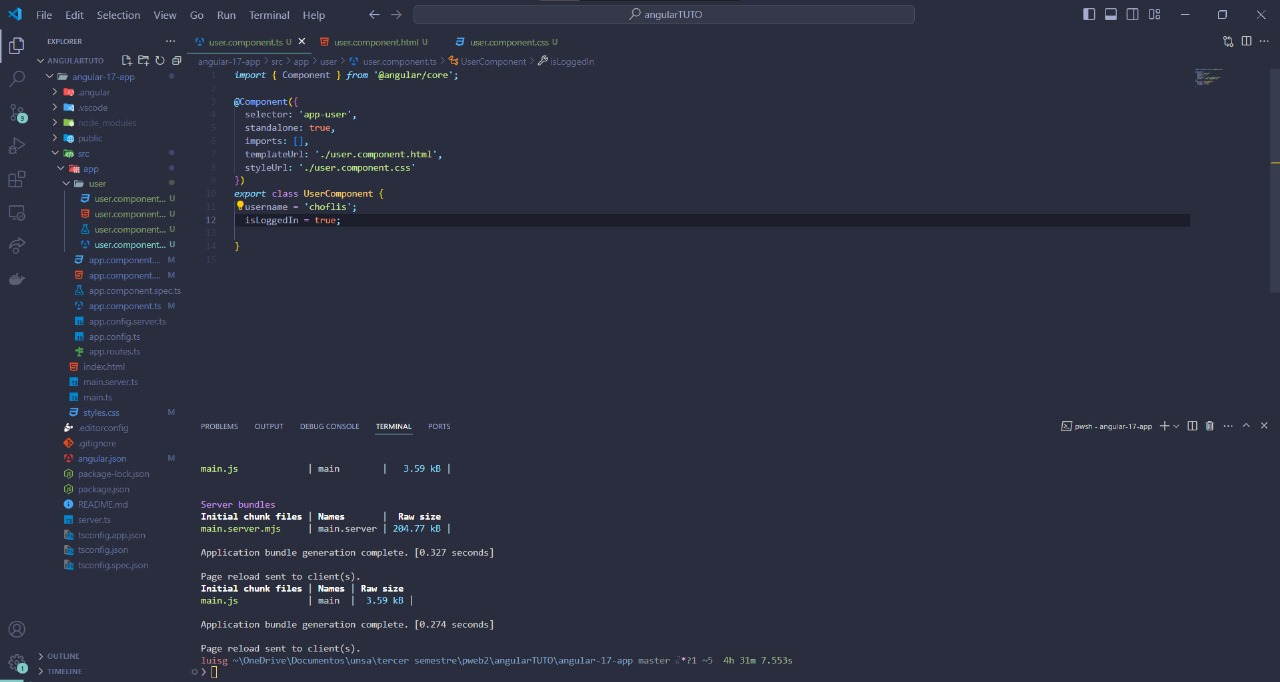
\includegraphics[width=0.8\textwidth,keepaspectratio]{img/creamosuncomponente.jpg}
			%\includesvg{img/automata.svg}
	
		\end{figure}
		\item Luego probaremos el servidor que crea angular, para que funcione un componente hijo en un componente padre este tiene que ser importado en el componente padre.
		\begin{figure}[H]
			\centering
			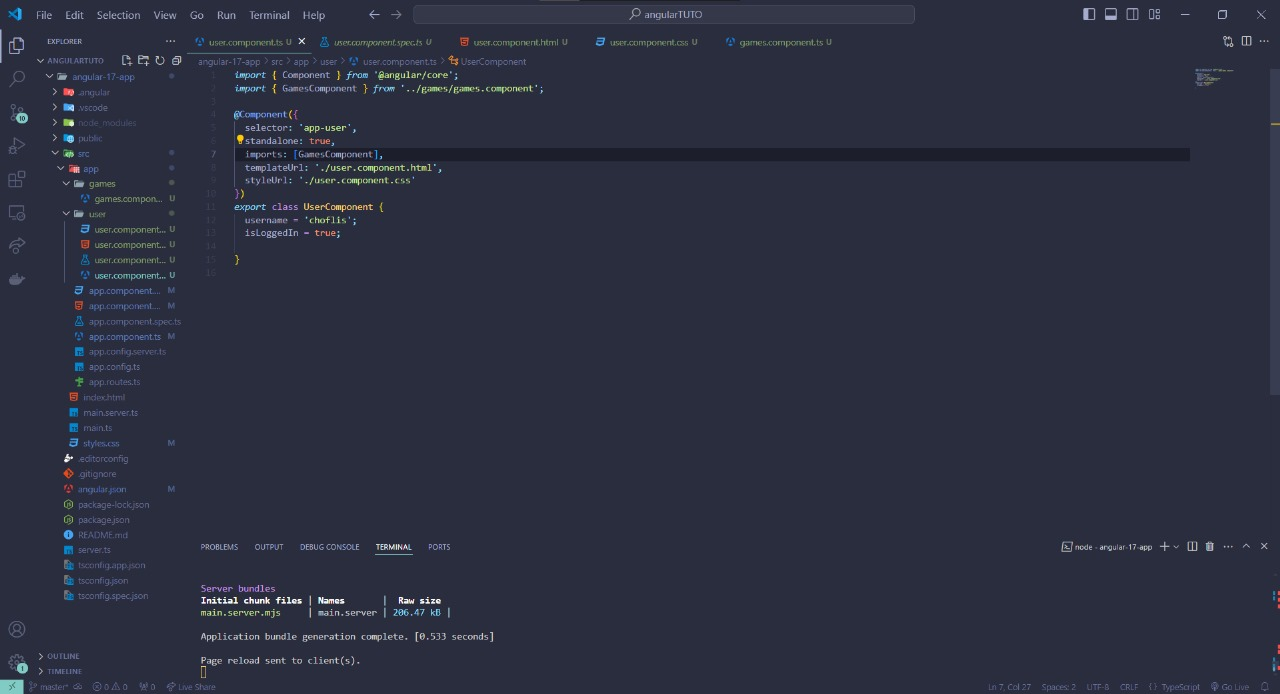
\includegraphics[width=0.8\textwidth,keepaspectratio]{img/tenemosqueimportarparausarloenotrocomponente.jpg}
			%\includesvg{img/automata.svg}
	
		\end{figure}
		\item ahora el comando para correr el servidor.
		\begin{lstlisting}[language=bash,caption={Comandos del servidor}][H]
			$ ng serve
			$ ng serve --open
		\end{lstlisting}
		\item Ahora podremos ver las modificaciones que hicimos
		\begin{figure}[H]
			\centering
			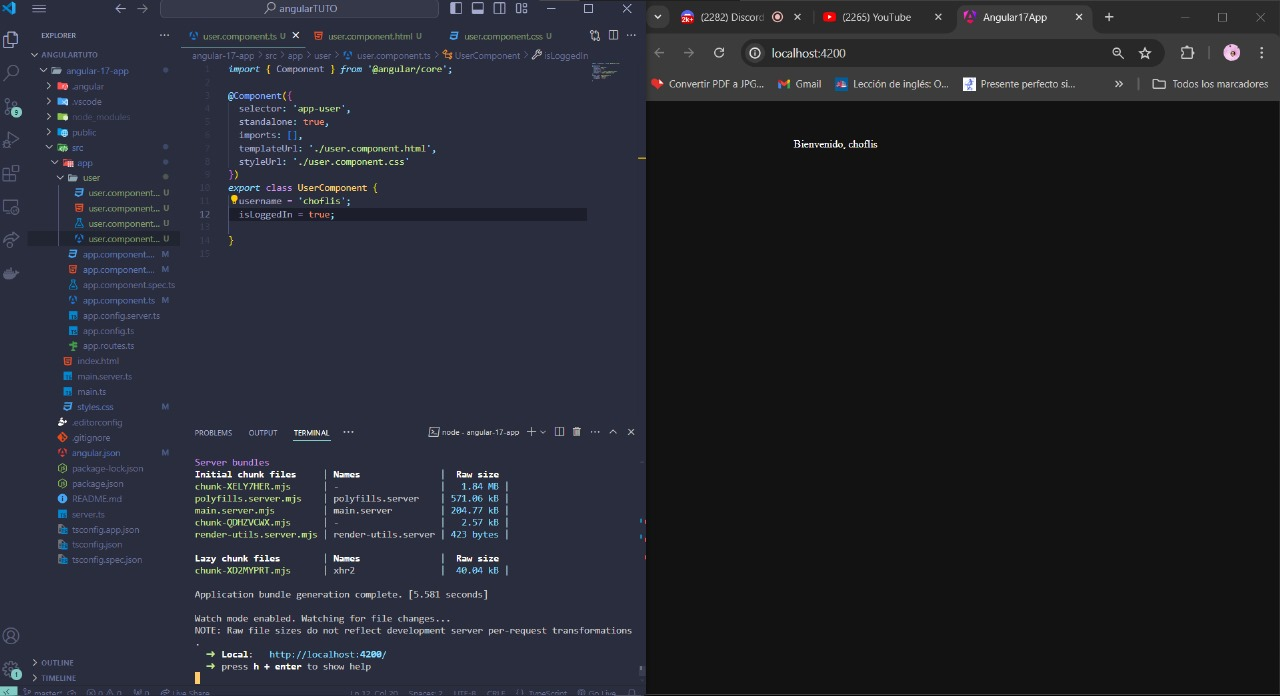
\includegraphics[width=0.8\textwidth,keepaspectratio]{img/servidorInicio.jpg}
			%\includesvg{img/automata.svg}
	
		\end{figure}
		\begin{figure}[H]
			\centering
			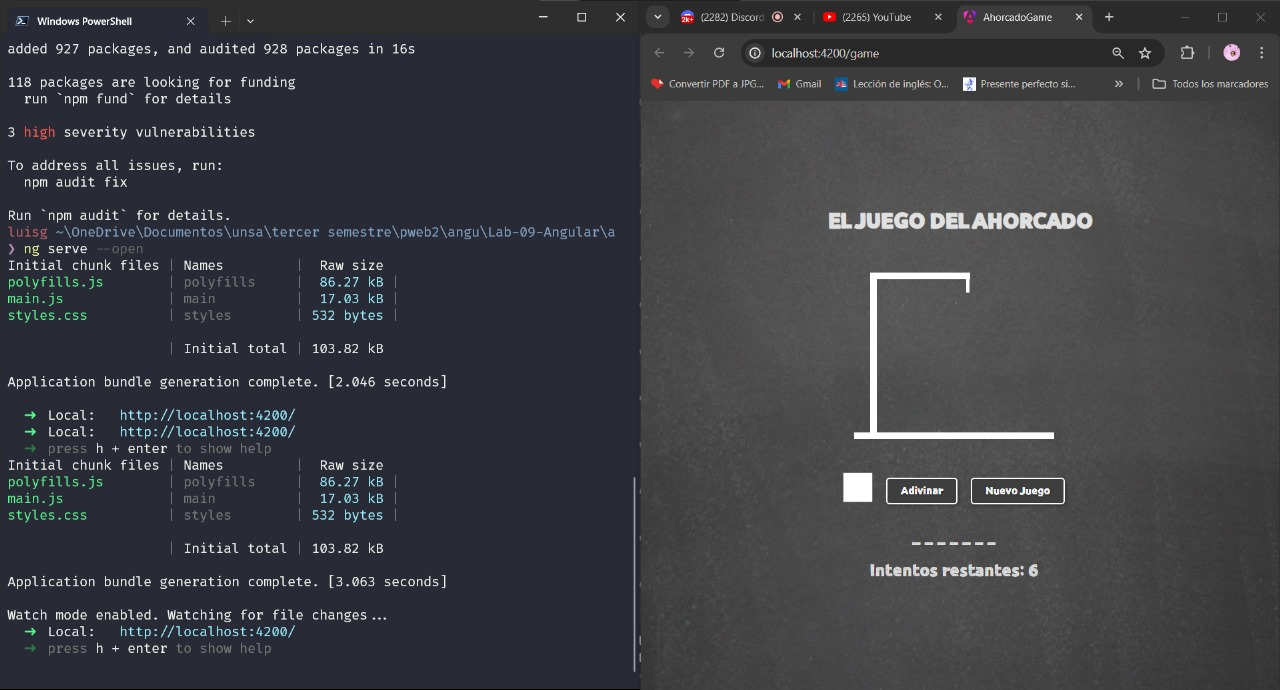
\includegraphics[width=0.8\textwidth,keepaspectratio]{img/iniciamos el servidor.jpg}
			%\includesvg{img/automata.svg}
	
		\end{figure}
		\item Inicialmente nos sale una página que nos da la bienvenida, pero como hicimos modificaciones nos aparece las páginas creadas.
		\item Podemos usar los componentes que necesitemos, en caso no requeramos de uno, usamos la siguiente linea de comandos.
		\begin{figure}[H]
			\centering
			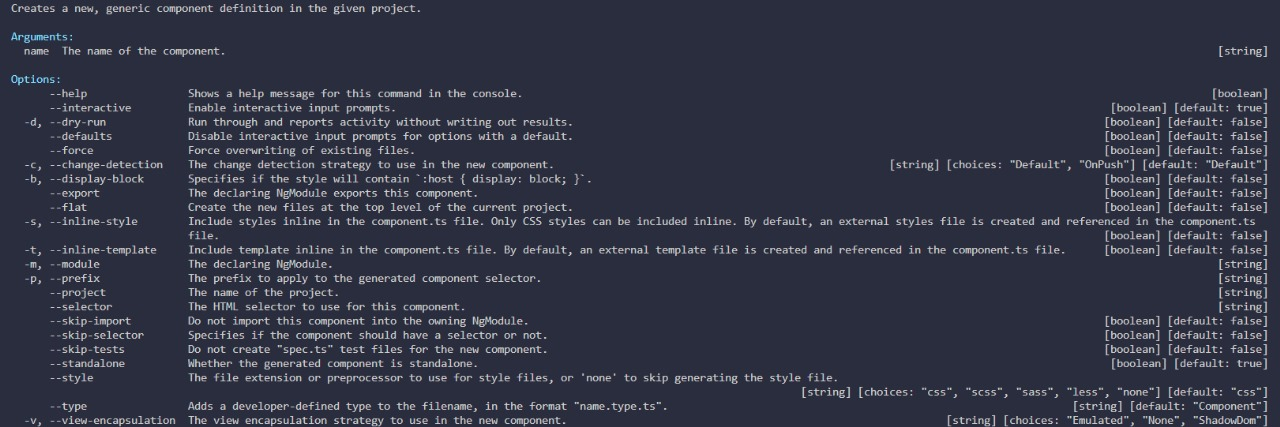
\includegraphics[width=0.8\textwidth,keepaspectratio]{img/comocrearcomponentes.jpg}
			%\includesvg{img/automata.svg}
	
		\end{figure}
		\item Ahora para las funciones de for o de if en angular tiene una sintaxis interesante ya que funcionan de la siguiente manera "@for" o "@if".
		\begin{figure}[H]
			\centering
			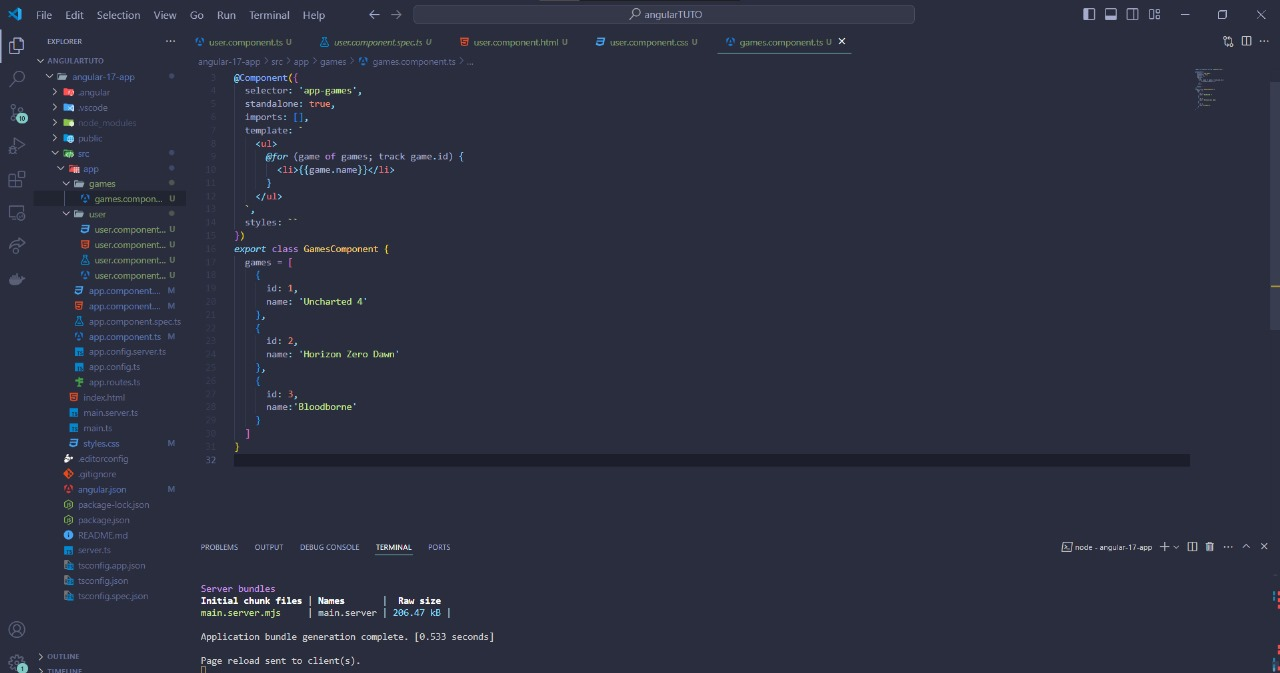
\includegraphics[width=0.8\textwidth,keepaspectratio]{img/comofuncionaforenAngular.jpg}
			%\includesvg{img/automata.svg}
	
		\end{figure}
		\begin{figure}[H]
			\centering
			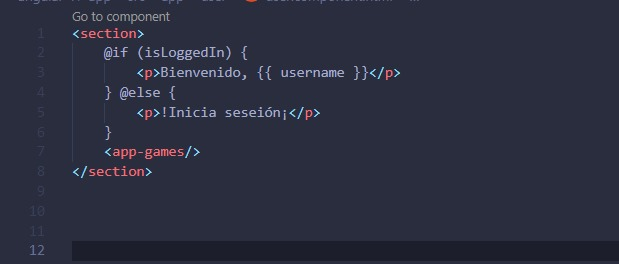
\includegraphics[width=0.8\textwidth,keepaspectratio]{img/paracolocarlousamosappgames.jpg}
			%\includesvg{img/automata.svg}
	
		\end{figure}
		\item Algo interesante de la ultima imagen es que para que un componente creado este en otro componente en el html tenemos que poner una referencia a ese componente en este caso la referencia es app-games.
		\item Por último podemos hacer que ocurran acciones como cuando damos un click o cosas asi, para esto necesitamos usar (click) dentro de nuestro código.
		\begin{figure}[H]
			\centering
			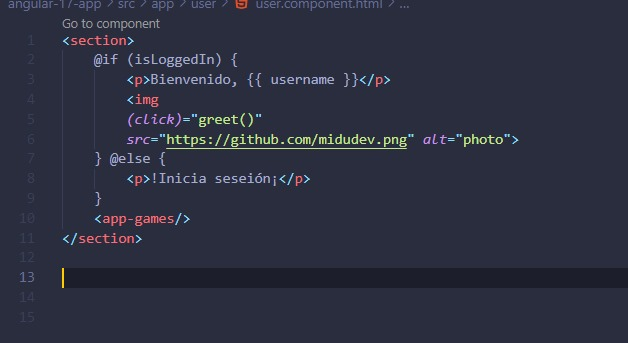
\includegraphics[width=0.8\textwidth,keepaspectratio]{img/accionesconunclick.jpg}
			%\includesvg{img/automata.svg}
	
		\end{figure}
	\end{itemize}

	\section{Ahorcado-Game}
	\begin{itemize}
		\item A continuacion se presenta la parte mas importante del codigo del juego Ahorcado-game.
		\item Primero se maneja la lógica central del juego del ahorcado. Esto incluye seleccionar una palabra aleatoria, llevar un registro de los intentos restantes, actualizar la palabra oculta según las letras adivinadas, y emitir eventos cuando cambian los intentos. Además, proporciona métodos para iniciar un nuevo juego y verificar si el juego ha terminado.
		
		\begin{figure}[H]
			\centering
			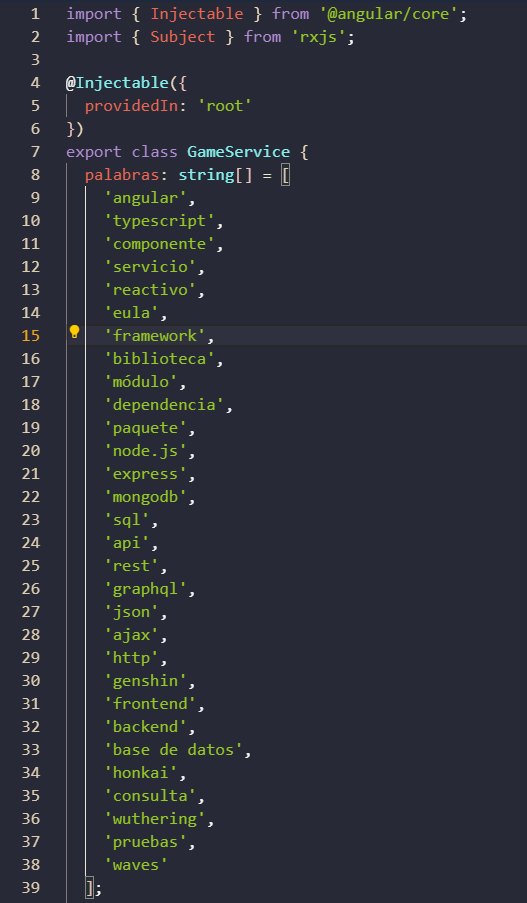
\includegraphics[width=0.4\textwidth,keepaspectratio]{img/game1.png}
			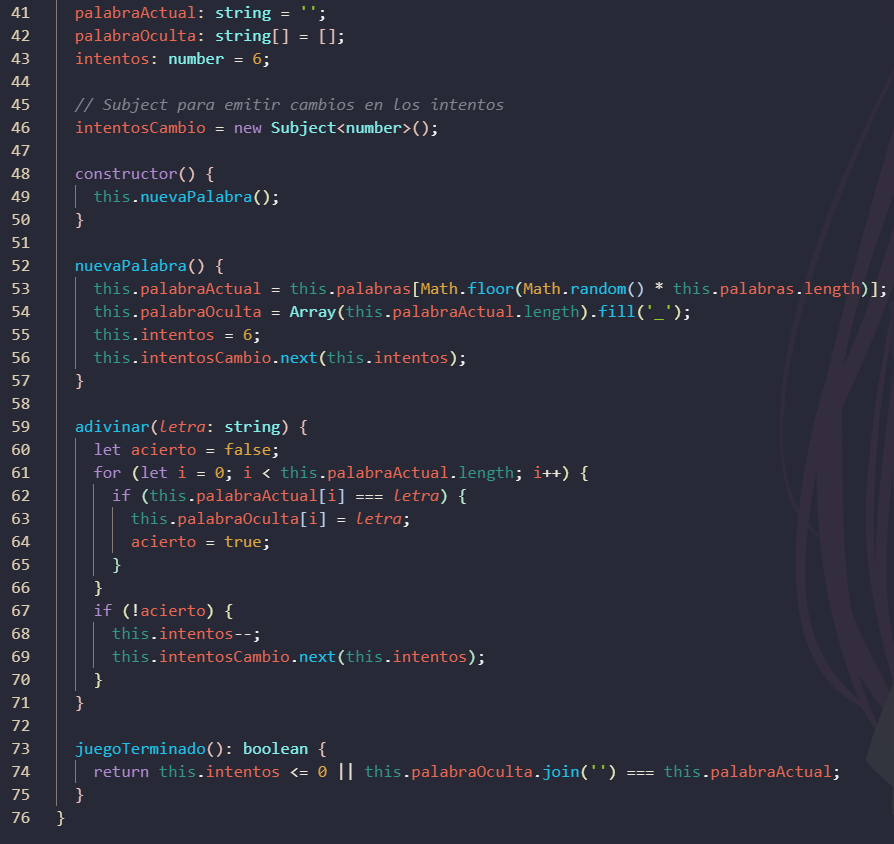
\includegraphics[width=0.5\textwidth,keepaspectratio]{img/game2.png}
		\end{figure}
		
		\item El siguiente codigo se encarga de mostrar las partes del cuerpo del muñeco del ahorcado en función de los intentos restantes. Se suscribe a los cambios en el número de intentos a través del GameService y actualiza la visibilidad de las partes del cuerpo en consecuencia. Utiliza clases CSS (hidden y visible) para controlar la visibilidad de los elementos en el DOM y ajusta el color de fondo para asegurarse de que las partes visibles tengan el color correcto.
		\begin{figure}[H]
			\centering
			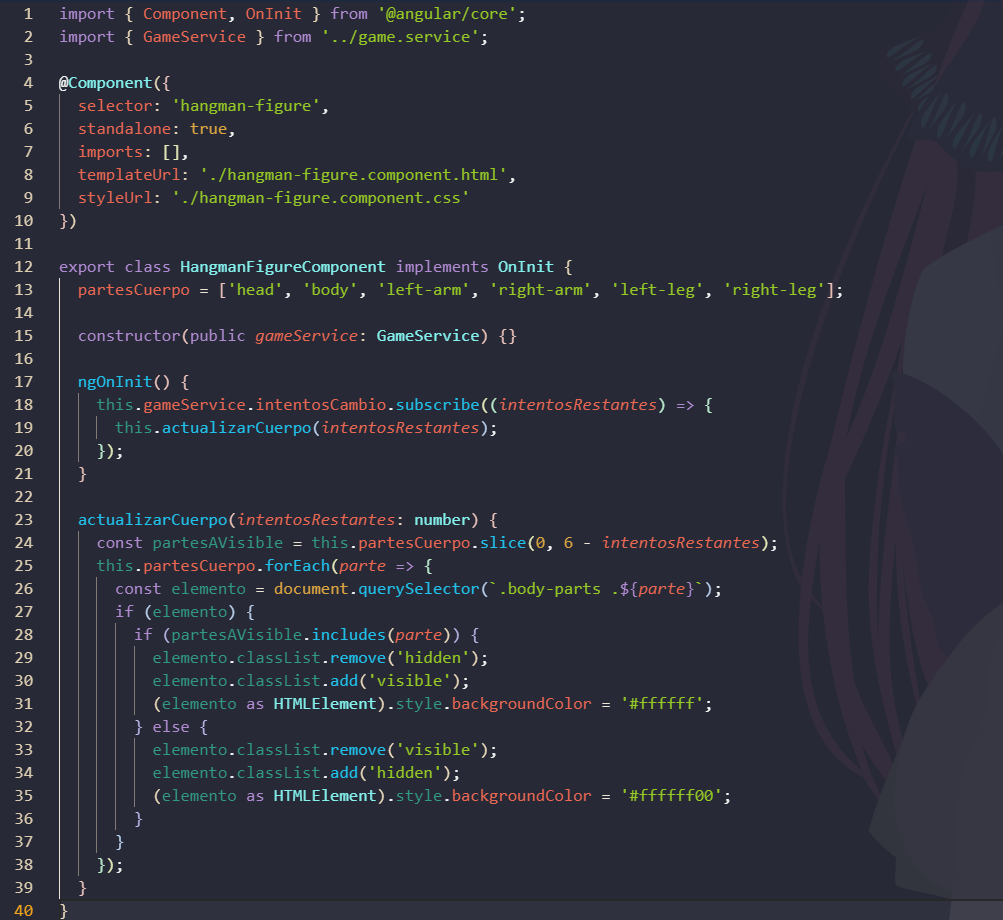
\includegraphics[width=0.8\textwidth,keepaspectratio]{img/game3.png}		
		\end{figure}
		
		\clearpage
		
		\item Por ultimo en cuanto al gameboard, el siguiente codigo es responsable de manejar la interfaz del juego del ahorcado. Proporciona un cuadro de entrada para que el usuario introduzca letras y botones para adivinar letras o iniciar un nuevo juego. Utiliza el GameService para manejar la lógica del juego, como verificar las letras adivinadas y generar nuevas palabras.
		
		\begin{figure}[H]
			\centering
			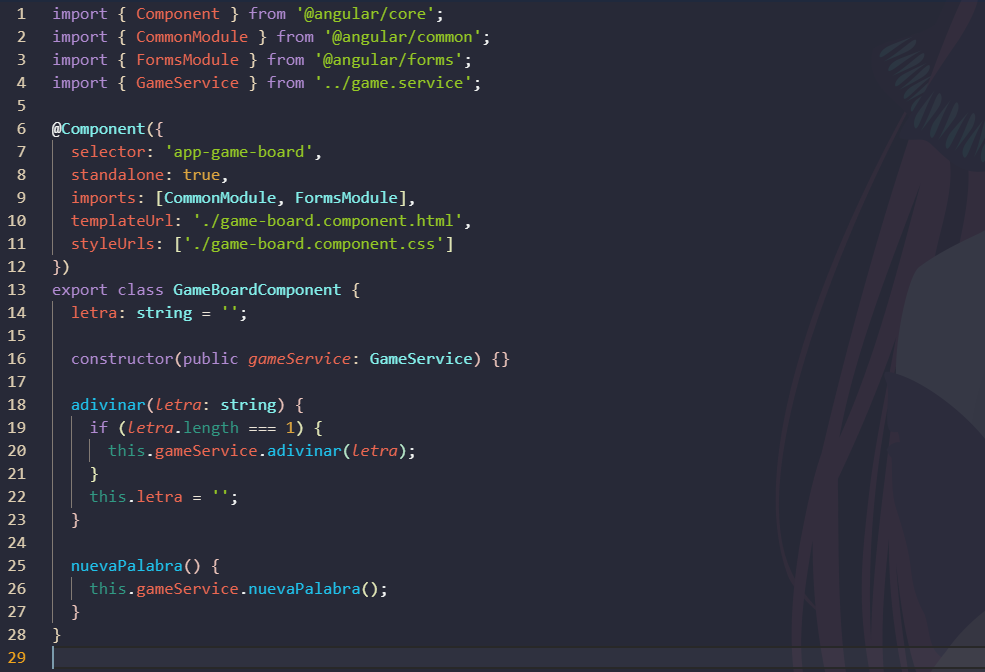
\includegraphics[width=0.8\textwidth,keepaspectratio]{img/game4.png}		
		\end{figure}
		
		
		
		
		
	\end{itemize}



\clearpage

	\section{\textcolor{red}{Rúbricas}}
	
	\subsection{\textcolor{red}{Entregable Informe}}
	\begin{table}[H]
		\caption{Tipo de Informe}
		\setlength{\tabcolsep}{0.5em} % for the horizontal padding
		{\renewcommand{\arraystretch}{1.5}% for the vertical padding
		\begin{tabular}{|p{3cm}|p{12cm}|}
			\hline
			\multicolumn{2}{|c|}{\textbf{\textcolor{red}{Informe}}}  \\
			\hline 
			\textbf{\textcolor{red}{Latex}} & \textcolor{blue}{El informe está en formato PDF desde Latex,  con un formato limpio (buena presentación) y facil de leer.}   \\ 
			\hline 
			
			
		\end{tabular}
	}
	\end{table}
	
	
	
	
	


\section{Referencias}
\begin{itemize}			
	\item Sobre Angular
	\item \url{https://docs.angular.lat/docs}
	\item \url{https://v2.angular.io/docs/ts/latest/guide/}
	\item \url{https://angular.dev/}
	\item \url{https://angular.dev/tutorials/learn-angular}
\end{itemize}	
	
%\clearpage
%\bibliographystyle{apalike}
%\bibliographystyle{IEEEtranN}
%\bibliography{bibliography}

\end{document}